\documentclass[crop,tikz]{standalone}

\tikzset{>=latex}
\colorlet{green}{black!40!green}
\newcommand{\F}{\vec{F}}

\begin{document}
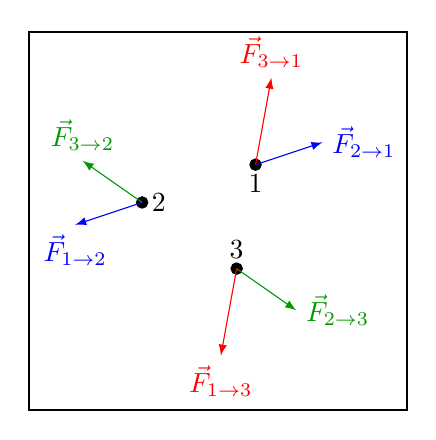
\begin{tikzpicture}[scale=1.2]
  \draw[thick] (-2,-2) -- ++(4,0) -- ++(0,4) -- ++(-4,0) -- cycle;
  \pgfmathsetmacro{\radi}{0.06};
  \pgfmathsetmacro{\xone}{0.4};
  \pgfmathsetmacro{\yone}{0.6};
  \pgfmathsetmacro{\xtwo}{-0.8};
  \pgfmathsetmacro{\ytwo}{0.2};
  \pgfmathsetmacro{\xthr}{0.2};
  \pgfmathsetmacro{\ythr}{-0.5};
  % coordinates
  \coordinate (r1) at (\xone,\yone);
  \coordinate (r2) at (\xtwo,\ytwo);
  \coordinate (r3) at (\xthr,\ythr);
  % distances
  \pgfmathsetmacro{\donetwo}{(\xone-\xtwo)^2 + (\yone-\ytwo)^(3/2)};
  \pgfmathsetmacro{\donethr}{(\xone-\xthr)^2 + (\yone-\ythr)^(3/2)};
  \pgfmathsetmacro{\dtwothr}{(\xtwo-\xthr)^2 + (\ytwo-\ythr)^(3/2)};
  % 1
  \draw[fill] (r1) circle (\radi) node[below] {$1$};
  \draw[->,blue] (r1) -- ++({(\xone-\xtwo)/\donetwo}, {(\yone-\ytwo)/\donetwo}) node[right] {$\F_{2\to 1}$};
  \draw[->,red]  (r1) -- ++({(\xone-\xthr)/\donethr}, {(\yone-\ythr)/\donethr}) node[above] {$\F_{3\to 1}$};
  % 2
  \draw[fill] (r2) circle (\radi) node[right] {$2$};
  \draw[->,blue]  (r2) -- ++({(\xtwo-\xone)/\donetwo}, {(\ytwo-\yone)/\donetwo}) node[below] {$\F_{1\to 2}$};
  \draw[->,green] (r2) -- ++({(\xtwo-\xthr)/\dtwothr}, {(\ytwo-\ythr)/\dtwothr}) node[above] {$\F_{3\to 2}$};
  % 3
  \draw[fill] (r3) circle (\radi) node[above] {$3$};
  \draw[->,red]   (r3) -- ++({(\xthr-\xone)/\donethr}, {(\ythr-\yone)/\donethr}) node[below] {$\F_{1\to 3}$};
  \draw[->,green] (r3) -- ++({(\xthr-\xtwo)/\dtwothr}, {(\ythr-\ytwo)/\dtwothr}) node[right] {$\F_{2\to 3}$};
\end{tikzpicture}
\end{document}
